\documentclass[12pt, a4paper]{article}

% --- Pakete ---
\usepackage[utf8]{inputenc}
\usepackage[T1]{fontenc}
% babel-german nicht installiert, daher weglassen
\usepackage{amsmath, amssymb}
\usepackage{graphicx}
\usepackage{hyperref}
\usepackage{listings}
\usepackage{xcolor}
\usepackage{geometry}
\usepackage{booktabs}
\usepackage{float}
\usepackage{enumitem}
\usepackage{tikz}
\usetikzlibrary{arrows.meta, positioning, shapes.geometric, fit, calc}

\geometry{margin=2.5cm}
\hypersetup{colorlinks=true, linkcolor=blue!60!black, urlcolor=blue!60!black}

\lstset{
    language=Python,
    basicstyle=\ttfamily\small,
    keywordstyle=\color{blue!70!black}\bfseries,
    commentstyle=\color{green!50!black}\itshape,
    stringstyle=\color{red!60!black},
    numbers=left,
    numberstyle=\tiny\color{gray},
    breaklines=true,
    frame=single,
    rulecolor=\color{gray!30},
    backgroundcolor=\color{gray!5},
    tabsize=4,
    showstringspaces=false,
}

\title{%
    \vspace{-1cm}
    \textbf{Transformer f\"ur Muon Track Reconstruction}\\[0.5em]
    \large Detaillierte Erkl\"arung der Architektur und aller Scripts\\[0.3em]
    \normalsize Basierend auf der iceaggr-Architektur (Inar Timiryasov)
}
\author{Generiert f\"ur Janik H.}
\date{M\"arz 2026}

\begin{document}
\maketitle
\tableofcontents
\newpage

% =====================================================================
\section{\"Uberblick: Was machen wir hier eigentlich?}
% =====================================================================

\subsection{Das Problem}
In IceCube detektieren wir Neutrinos, indem wir das Cherenkov-Licht messen,
das entsteht, wenn ein Neutrino mit dem Eis interagiert und dabei ein Muon
erzeugt. Dieses Muon fliegt durch den Detektor und erzeugt dabei Lichtblitze
an den optischen Modulen (DOMs).

\textbf{Unser Ziel:} Aus den gemessenen Lichtpulsen (wann hat welcher DOM
wie viel Licht gesehen?) die \textbf{Flugrichtung des Muons} rekonstruieren.
Die Richtung wird beschrieben durch zwei Winkel:
\begin{itemize}
    \item \textbf{Zenith} ($\theta$): Winkel zur vertikalen Achse ($0^\circ$ = von oben, $180^\circ$ = von unten)
    \item \textbf{Azimuth} ($\phi$): Winkel in der horizontalen Ebene ($0^\circ$--$360^\circ$)
\end{itemize}

\subsection{Warum ein Transformer?}
Bisher haben wir Graph Neural Networks (GNNs, z.B. DynEdge) benutzt.
Ein Transformer hat aber einige Vorteile:
\begin{itemize}
    \item \textbf{Globale Aufmerksamkeit:} Jeder DOM kann direkt auf jeden anderen DOM schauen --
          bei GNNs muss die Information \"uber mehrere Schichten propagieren.
    \item \textbf{Einfachere Architektur:} Keine Graph-Konstruktion (k-NN) n\"otig.
    \item \textbf{Skalierbarkeit:} Transformer sind gut erforscht und optimiert (Flash Attention).
\end{itemize}

\subsection{Der Datenfluss (Big Picture)}

\begin{center}
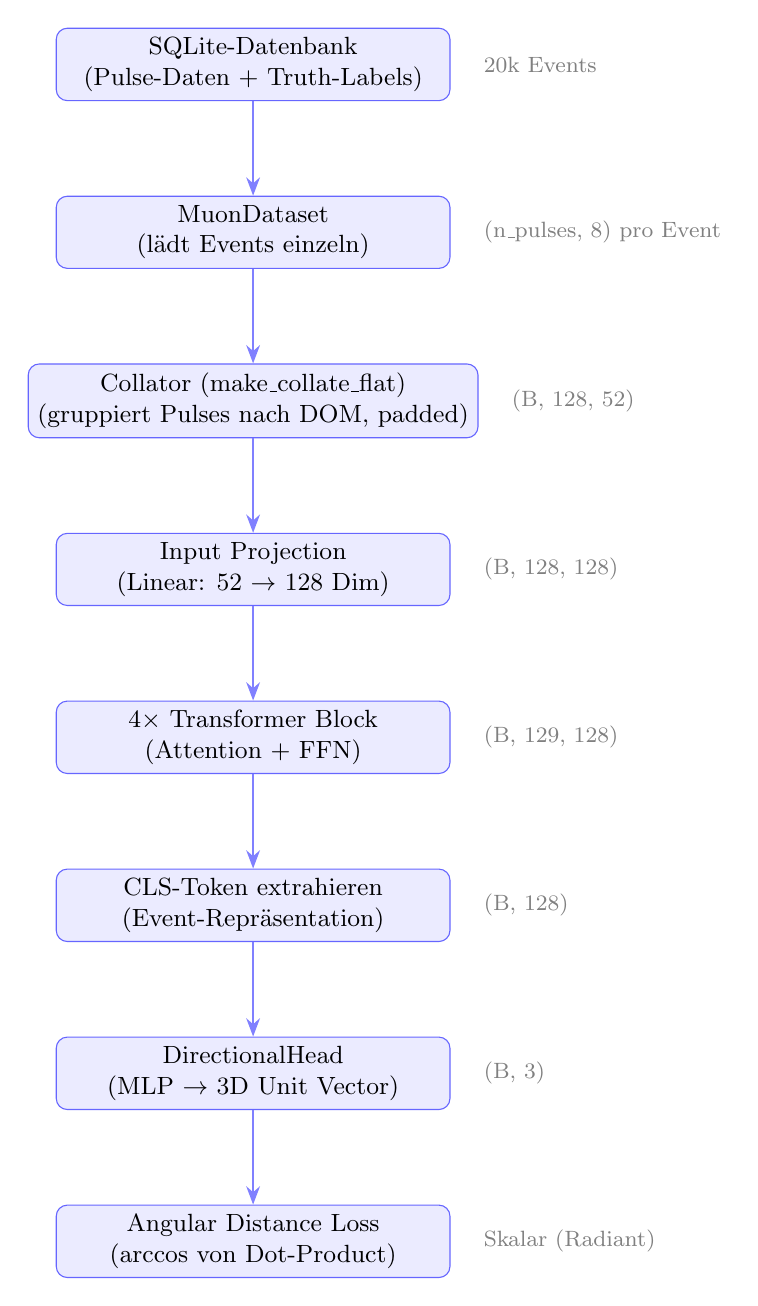
\begin{tikzpicture}[
    node distance=1.2cm,
    box/.style={rectangle, draw=blue!60, fill=blue!8, rounded corners,
                minimum width=5cm, minimum height=0.9cm, align=center,
                font=\small},
    arrow/.style={-Stealth, thick, draw=blue!50},
]
    \node[box] (db) {SQLite-Datenbank\\(Pulse-Daten + Truth-Labels)};
    \node[box, below=of db] (dataset) {MuonDataset\\(l\"adt Events einzeln)};
    \node[box, below=of dataset] (collator) {Collator (make\_collate\_flat)\\(gruppiert Pulses nach DOM, padded)};
    \node[box, below=of collator] (proj) {Input Projection\\(Linear: 52 $\to$ 128 Dim)};
    \node[box, below=of proj] (transformer) {4$\times$ Transformer Block\\(Attention + FFN)};
    \node[box, below=of transformer] (cls) {CLS-Token extrahieren\\(Event-Repr\"asentation)};
    \node[box, below=of cls] (head) {DirectionalHead\\(MLP $\to$ 3D Unit Vector)};
    \node[box, below=of head] (loss) {Angular Distance Loss\\(arccos von Dot-Product)};

    \draw[arrow] (db) -- (dataset);
    \draw[arrow] (dataset) -- (collator);
    \draw[arrow] (collator) -- (proj);
    \draw[arrow] (proj) -- (transformer);
    \draw[arrow] (transformer) -- (cls);
    \draw[arrow] (cls) -- (head);
    \draw[arrow] (head) -- (loss);

    % Annotations
    \node[right=0.3cm of db, font=\footnotesize\color{gray}] {20k Events};
    \node[right=0.3cm of dataset, font=\footnotesize\color{gray}] {(n\_pulses, 8) pro Event};
    \node[right=0.3cm of collator, font=\footnotesize\color{gray}] {(B, 128, 52)};
    \node[right=0.3cm of proj, font=\footnotesize\color{gray}] {(B, 128, 128)};
    \node[right=0.3cm of transformer, font=\footnotesize\color{gray}] {(B, 129, 128)};
    \node[right=0.3cm of cls, font=\footnotesize\color{gray}] {(B, 128)};
    \node[right=0.3cm of head, font=\footnotesize\color{gray}] {(B, 3)};
    \node[right=0.3cm of loss, font=\footnotesize\color{gray}] {Skalar (Radiant)};
\end{tikzpicture}
\end{center}


% =====================================================================
\newpage
\section{Die Daten-Pipeline}
% =====================================================================

\subsection{Die Datenbank (SQLite)}

Unsere Daten liegen in einer SQLite-Datenbank mit zwei Tabellen:

\begin{table}[H]
\centering
\begin{tabular}{lll}
\toprule
\textbf{Tabelle} & \textbf{Wichtige Spalten} & \textbf{Bedeutung} \\
\midrule
\texttt{SplitInIcePulses} & \texttt{dom\_x, dom\_y, dom\_z} & Position des DOMs (Meter) \\
& \texttt{dom\_time} & Ankunftszeit des Lichts (ns) \\
& \texttt{charge} & Gemessene Ladung (PE) \\
& \texttt{hlc} & Hard Local Coincidence (0 oder 1) \\
& \texttt{string, dom\_number} & Welcher String, welcher DOM \\
& \texttt{event\_no} & Zu welchem Event geh\"ort der Puls \\
\midrule
\texttt{truth} & \texttt{zenith, azimuth} & Wahre Muon-Richtung (Radiant) \\
& \texttt{energy} & Wahre Energie (GeV) \\
& \texttt{event\_no} & Event-Nummer \\
\bottomrule
\end{tabular}
\caption{Aufbau der SQLite-Datenbank}
\end{table}

Ein \textbf{Event} besteht aus vielen Pulsen (typischerweise 20--500), weil
das Muon an vielen DOMs Licht erzeugt. Jeder Puls ist eine Zeile in
\texttt{SplitInIcePulses}.

\subsection{MuonDataset (\texttt{data/dataset.py})}

Das Dataset l\"adt ein Event nach dem anderen aus der Datenbank:

\begin{lstlisting}[caption={MuonDataset -- vereinfacht}]
class MuonDataset(Dataset):
    def __init__(self, db_path):
        # Alle event_nos aus truth-Tabelle laden
        self.event_nos = [...]  # z.B. [1, 2, 3, ..., 20093]

    def __getitem__(self, idx):
        event_no = self.event_nos[idx]
        # Pulse laden: SELECT dom_x, dom_y, ... WHERE event_no = ?
        pulse_features = ...  # Shape: (n_pulses, 8)
        # Truth laden: SELECT zenith, azimuth WHERE event_no = ?
        target = angles_to_unit_vector(zenith, azimuth)  # (3,)
        return {"pulse_features": ..., "target": ..., ...}
\end{lstlisting}

\textbf{Wichtig:} Jeder Worker im DataLoader \"offnet seine eigene
Datenbank-Connection (wegen Multi-Processing). Die DB wird im Read-Only-Modus
ge\"offnet (\texttt{?mode=ro\&immutable=1}).

\textbf{Target-Konvertierung:} Statt Zenith/Azimuth als Winkel zu predicten,
konvertieren wir sie in einen \textbf{3D-Einheitsvektor}:
\begin{align}
    x &= \sin(\theta) \cdot \cos(\phi) \\
    y &= \sin(\theta) \cdot \sin(\phi) \\
    z &= \cos(\theta)
\end{align}
Das ist besser, weil Winkel Periodizit\"atsprobleme haben (z.B. ist $0^\circ = 360^\circ$
f\"ur Azimuth, was der Loss-Funktion Schwierigkeiten macht).

\subsection{Der Collator (\texttt{data/collators.py})}

\textbf{Problem:} Jedes Event hat eine unterschiedliche Anzahl Pulses
(variable L\"ange). F\"ur den Transformer brauchen wir aber einen festen
Tensor pro Batch.

\textbf{L\"osung des Collators (angelehnt an iceaggr):}

Der Collator gruppiert die Pulses \textbf{nach DOM} statt sie einzeln zu behandeln.
Das ist clever, weil:
\begin{itemize}
    \item Ein DOM typischerweise mehrere Pulses hat (Nachleuchten, Rauschen)
    \item Die DOM-Position nur einmal gespeichert werden muss
    \item Die Sequenzl\"ange von ``Anzahl Pulses'' auf ``Anzahl DOMs'' reduziert wird
\end{itemize}

\subsubsection{Schritt f\"ur Schritt}

\begin{enumerate}[label=\textbf{Schritt \arabic*:}]

\item \textbf{Sensor-ID berechnen:}
Jeder DOM wird identifiziert durch \texttt{string * 60 + dom\_number}.
Das ergibt eine eindeutige Sensor-ID (0--5159).

\item \textbf{Pulses nach DOM gruppieren:}
Alle Pulses mit der gleichen (Event, Sensor-ID)-Kombination geh\"oren
zum selben DOM im selben Event.

\item \textbf{Maximal K Pulses pro DOM:}
Pro DOM werden nur die ersten $K = 16$ Pulses behalten (nach Ankunftszeit
sortiert). Das begrenzt die Daten pro DOM.

\item \textbf{Pulse-Features normalisieren:}
\begin{itemize}
    \item Zeit: $(t - 10000) / 30000$ \quad (typische Zeiten: 5000--40000\,ns)
    \item Charge: $\log_{10}(\text{charge}) / 3$ \quad (typisch: 0.1--1000\,PE)
    \item HLC: $\text{hlc} - 0.5$ \quad (0/1 $\to$ $-0.5$/$+0.5$)
\end{itemize}

\item \textbf{DOM-Vektor zusammenbauen:}
F\"ur jeden DOM wird ein flacher Vektor gebaut:
\[
    \mathbf{v}_\text{DOM} = [\underbrace{x, y, z}_\text{Position}, \underbrace{\log(n)}_\text{Anzahl Pulses}, \underbrace{t_1, q_1, h_1, \ldots, t_K, q_K, h_K}_\text{K Pulse-Triplets}]
\]
Dimension: $4 + 3 \times K = 4 + 3 \times 16 = 52$.

Die Position $(x, y, z)$ kommt aus einer vorberechneten \textbf{Geometry-Tabelle}
(normalisiert auf $\approx [-1, 1]$), nicht aus den Pulse-Features!

\item \textbf{Auf max\_doms padden:}
Jedes Event wird auf genau $128$ DOMs gepaddet (mit Nullen).
Eine \textbf{Padding-Mask} (Bool-Tensor) markiert, welche DOMs echt sind.

Falls ein Event mehr als 128 DOMs hat, werden die mit der \textbf{sp\"atesten
Ankunftszeit} verworfen (die fr\"uhesten sind informativer).

\end{enumerate}

\textbf{Output des Collators:}
\begin{itemize}
    \item \texttt{dom\_vectors}: Shape $(B, 128, 52)$ -- die DOM-Feature-Vektoren
    \item \texttt{padding\_mask}: Shape $(B, 128)$ -- True = echte DOMs
    \item \texttt{targets}: Shape $(B, 3)$ -- die wahren Richtungs-Unit-Vektoren
\end{itemize}


% =====================================================================
\newpage
\section{Der Transformer (Modell-Architektur)}
% =====================================================================

\subsection{Was ist ein Transformer? (Ganz einfach)}

Ein Transformer ist ein Modell, das eine \textbf{Sequenz} von Vektoren
verarbeitet. In unserem Fall ist die Sequenz: die $N$ DOMs eines Events.

Die Kernidee: \textbf{Self-Attention} -- jeder DOM darf ``alle anderen DOMs
anschauen'' und entscheiden, welche Information wichtig ist.

\textbf{Analogie:} Stell dir eine Gruppe von Leuten vor (DOMs). Jede Person
hat eine Information. In einer Besprechung (Attention) kann jeder jeden
fragen und die wichtigsten Antworten zusammenfassen.

\subsection{Eingabe: Input Projection}

Der Collator gibt uns DOM-Vektoren der Dimension 52. Der Transformer arbeitet
aber intern mit Dimension $d_\text{model} = 128$. Also brauchen wir eine
Projektion:
\[
    \mathbf{h}^{(0)} = W_\text{proj} \cdot \mathbf{v}_\text{DOM} \qquad
    W_\text{proj} \in \mathbb{R}^{128 \times 52}
\]

Das ist einfach eine lineare Transformation (Matrix-Multiplikation) ohne Bias.
Optional kann man ein MLP (2 Schichten mit GELU) benutzen.

Danach kommt \textbf{RMSNorm} (siehe unten).

\subsection{CLS-Token: Das ``Zusammenfassungs-Token''}

\textbf{Problem:} Der Transformer gibt einen Vektor \textit{pro DOM} aus.
Wir brauchen aber \textit{einen} Vektor f\"ur das ganze Event.

\textbf{L\"osung:} Wir f\"ugen ein spezielles Token am Anfang der Sequenz
hinzu -- das \textbf{CLS-Token} (Classification Token). Es ist ein
lernbarer Vektor $\mathbf{c} \in \mathbb{R}^{128}$.

Die Sequenz wird also:
\[
    [\mathbf{c}, \mathbf{h}_1, \mathbf{h}_2, \ldots, \mathbf{h}_N]
\]

Im Transformer kann das CLS-Token \"uber Attention alle DOMs ``anschauen''
und ihre Information aggregieren. Am Ende nehmen wir nur das CLS-Token
als Event-Repr\"asentation.

\textbf{Analogie:} Das CLS-Token ist wie ein Moderator, der bei der
Besprechung zuh\"ort und am Ende eine Zusammenfassung schreibt.

\subsection{RMSNorm (Root Mean Square Normalization)}

Normalisierung stabilisiert das Training. RMSNorm ist einfacher als
LayerNorm (kein Mean-Shift):
\[
    \text{RMSNorm}(\mathbf{x}) = \frac{\mathbf{x}}{\sqrt{\frac{1}{d}\sum_{i=1}^d x_i^2}}
\]

Das skaliert den Vektor so, dass sein RMS-Wert 1 ist. \textbf{Keine
lernbaren Parameter} (anders als bei LayerNorm, das noch $\gamma$ und
$\beta$ hat).

\textbf{Warum?} Weniger Parameter, schneller, und funktioniert genauso gut.

\subsection{Self-Attention mit QK-Norm}

Das ist das Herzst\"uck des Transformers. Hier wird entschieden, welche
DOMs aufeinander ``achten''.

\subsubsection{Die drei Projektionen: Q, K, V}

Jeder DOM-Vektor $\mathbf{h}$ wird dreimal projiziert:
\begin{align}
    \mathbf{q} &= W_Q \cdot \mathbf{h} \quad \text{(Query -- ``Was suche ich?'')} \\
    \mathbf{k} &= W_K \cdot \mathbf{h} \quad \text{(Key -- ``Was biete ich an?'')} \\
    \mathbf{v} &= W_V \cdot \mathbf{h} \quad \text{(Value -- ``Meine eigentliche Information'')}
\end{align}

\textbf{Analogie:}
\begin{itemize}
    \item \textbf{Query:} Du gehst in eine Bibliothek und sagst: ``Ich suche etwas \"uber Physik''
    \item \textbf{Key:} Jedes Buch hat einen Titel (Key)
    \item \textbf{Value:} Der Inhalt des Buchs
    \item \textbf{Attention:} Die B\"ucher, deren Titel am besten zu deiner Suche passt,
          bekommst du am meisten Gewicht
\end{itemize}

\subsubsection{Attention-Berechnung}

\begin{enumerate}
\item \textbf{Dot-Product:} $\text{score}_{ij} = \mathbf{q}_i \cdot \mathbf{k}_j / \sqrt{d_\text{head}}$

Das Skalarprodukt misst, wie \"ahnlich Query $i$ und Key $j$ sind.
Division durch $\sqrt{d_\text{head}}$ verhindert, dass die Werte zu gross werden.

\item \textbf{QK-Norm:} Vor dem Dot-Product werden Q und K mit RMSNorm normalisiert.
Das macht das Training stabiler, besonders in tiefen Modellen.

\item \textbf{Masking:} Padding-DOMs (die nicht existieren) bekommen $-\infty$ als Score,
damit sie nach Softmax Gewicht 0 bekommen.

\item \textbf{Softmax:} $\alpha_{ij} = \text{softmax}_j(\text{scores}_i)$

Konvertiert Scores in Wahrscheinlichkeiten (summe = 1).

\item \textbf{Gewichtete Summe:} $\mathbf{o}_i = \sum_j \alpha_{ij} \cdot \mathbf{v}_j$

Der Output f\"ur DOM $i$ ist die gewichtete Summe aller Values.

\item \textbf{Output-Projektion:} $\text{out} = W_\text{proj} \cdot \mathbf{o}$
\end{enumerate}

\subsubsection{Multi-Head Attention}

Statt eine grosse Attention zu berechnen, teilen wir die Dimension in
$H = 8$ \textbf{Heads} auf. Jeder Head hat Dimension $d_\text{head} = 128/8 = 16$.

\textbf{Warum?} Verschiedene Heads k\"onnen verschiedene Dinge lernen:
\begin{itemize}
    \item Head 1: ``Welche DOMs sind r\"aumlich nah?''
    \item Head 2: ``Welche DOMs haben \"ahnliche Zeiten?''
    \item Head 3: ``Welche DOMs haben hohe Ladung?''
    \item etc.
\end{itemize}

\subsection{Feed-Forward Network (FFN) mit ReLU\textsuperscript{2}}

Nach der Attention kommt ein FFN -- zwei lineare Schichten mit einer
Aktivierungsfunktion dazwischen:
\[
    \text{FFN}(\mathbf{x}) = W_2 \cdot \text{ReLU}(W_1 \cdot \mathbf{x})^2
\]

\textbf{ReLU\textsuperscript{2}} bedeutet: erst ReLU (negative Werte = 0),
dann quadrieren. Das erzeugt eine \textbf{sparsere} Aktivierung als GELU
(mehr Werte werden exakt 0), was bei kleinen Modellen hilft.

Dimensionen: $128 \to 256 \to 128$.

\subsection{Ein Transformer-Block (Zusammen)}

Ein Block besteht aus:
\[
    \mathbf{x} = \mathbf{x} + \text{Attention}(\text{RMSNorm}(\mathbf{x}))
\]
\[
    \mathbf{x} = \mathbf{x} + \text{FFN}(\text{RMSNorm}(\mathbf{x}))
\]

Das ``$+$'' ist die \textbf{Residual Connection} -- der Input wird zum
Output addiert. Das hilft beim Gradient-Flow (Gradienten k\"onnen direkt
durchfliessen ohne durch Attention/FFN gehen zu m\"ussen).

\textbf{Pre-Norm:} Die Normalisierung kommt \textit{vor} der Attention/FFN
(nicht danach). Das ist stabiler beim Training.

\subsection{Residual Scaling + x0 Skip Connection}

Wir haben 4 Blocks. Vor jedem Block werden die Residuals skaliert:
\[
    \mathbf{x} = \lambda_\text{resid}^{(i)} \cdot \mathbf{x} + \lambda_\text{x0}^{(i)} \cdot \mathbf{x}_0
\]

wobei $\mathbf{x}_0$ der \textit{initiale} Zustand nach der Input-Projektion ist.

\begin{itemize}
    \item $\lambda_\text{resid}$ startet bei 1.0 (normales Residual)
    \item $\lambda_\text{x0}$ startet bei 0.1 (schwacher Skip zum Anfang)
    \item Beide sind \textbf{lernbar} (ein Skalar pro Layer)
\end{itemize}

\textbf{Warum?} In tiefen Transformer kann die Information vom Anfang
``vergessen'' werden. Die x0-Skip-Connection stellt sicher, dass die
originalen DOM-Features immer noch verf\"ugbar sind.

\subsection{Weight-Initialisierung}

Die Initialisierung der Gewichte ist wichtig f\"ur stabiles Training:

\begin{itemize}
    \item \textbf{Q, K, V, FFN-Input:} Uniform $\sim \mathcal{U}(-s, s)$ mit
          $s = \sqrt{3} \cdot d_\text{model}^{-0.5} \approx 0.153$
    \item \textbf{Output-Projektionen:} \textbf{Zero-Init!} ($W = 0$)

    Das bedeutet: Am Anfang des Trainings machen Attention und FFN
    \textit{gar nichts} (Output = 0), und die Residual Connection leitet
    den Input einfach durch. Das Modell lernt dann langsam, was es
    hinzuf\"ugen soll.
    \item \textbf{CLS-Token:} Normal $\sim \mathcal{N}(0, 0.02)$
\end{itemize}


% =====================================================================
\newpage
\section{Der Prediction Head (\texttt{models/directional\_head.py})}
% =====================================================================

Der DirectionalHead nimmt das CLS-Token (Dimension 128) und sagt die
Muon-Richtung als 3D-Einheitsvektor voraus:

\[
    \mathbf{d} = \text{normalize}\big(\underbrace{W_2 \cdot \text{GELU}(W_1 \cdot \mathbf{h}_\text{CLS})}_\text{MLP mit einer Hidden-Schicht}\big)
\]

Dimensionen: $128 \to 128 \to 3 \to \text{L2-Norm}$.

\textbf{L2-Normalisierung:} Der Output wird auf L\"ange 1 normalisiert:
\[
    \hat{\mathbf{d}} = \frac{\mathbf{d}}{||\mathbf{d}||_2}
\]

Das stellt sicher, dass der Output immer auf der Einheitskugel liegt
(ein g\"ultiger Richtungsvektor).

\textbf{Warum GELU statt ReLU\textsuperscript{2}?} Der Head ist klein
(nur 2 Schichten), da braucht man keine Sparsity. GELU ist ``glatter''
als ReLU und funktioniert besser f\"ur kleine MLPs.


% =====================================================================
\section{Die Loss-Funktion (\texttt{models/losses.py})}
% =====================================================================

\subsection{Angular Distance Loss}

Wir messen den Fehler als \textbf{Winkelabstand} (Opening Angle) zwischen
dem vorhergesagten und dem wahren Richtungsvektor:

\[
    \mathcal{L} = \frac{1}{B} \sum_{i=1}^{B} \arccos\big(\hat{\mathbf{d}}_i \cdot \mathbf{d}_i^{\text{true}}\big)
\]

\textbf{Schritt f\"ur Schritt:}
\begin{enumerate}
    \item Dot-Product: $s = \hat{\mathbf{d}} \cdot \mathbf{d}^{\text{true}}$
          \quad (Skalarprodukt zweier Einheitsvektoren = Cosinus des Winkels)
    \item Clipping: $s_\text{clip} = \text{clamp}(s, -0.9999, 0.9999)$
          \quad (arccos explodiert bei genau $\pm 1$)
    \item Winkel: $\alpha = \arccos(s_\text{clip})$ \quad (in Radiant)
    \item Mittelwert: $\mathcal{L} = \text{mean}(\alpha)$
\end{enumerate}

\textbf{Baseline:} Ein zuf\"allig ratender Predictor hat einen mittleren
Opening Angle von ${\sim}\,90^\circ$ ($\pi/2$ Radiant). Alles unter ${\sim}\,20^\circ$ ist
schon ziemlich gut.

\textbf{Warum nicht MSE auf Winkel?} MSE auf Azimuth hat ein Periodizit\"atsproblem
(der Abstand zwischen $1^\circ$ und $359^\circ$ w\"are $358^\circ$ statt $2^\circ$). Die Angular
Distance auf Unit-Vektoren hat dieses Problem nicht.


% =====================================================================
\newpage
\section{Das Training-Script (\texttt{scripts/train\_transformer.py})}
% =====================================================================

\subsection{\"Uberblick}

\begin{lstlisting}[caption={Trainings-Ablauf (Pseudo-Code)},language={}]
1. Geometry laden (DOM-Positionen)
2. Dataset erstellen (aus SQLite-DB)
3. Train/Val/Test Split (80/10/10)
4. Collator erstellen (mit Geometry)
5. Modell + Optimizer + Scheduler erstellen
6. Training Loop:
   - Fuer jede Epoche:
     - Training: Forward -> Loss -> Backward -> Update
     - Validation: Forward -> Metriken berechnen
     - Early Stopping pruefen
7. Bestes Modell laden, auf Test-Set evaluieren
8. Ergebnisse speichern
\end{lstlisting}

\subsection{Geometry laden}

Die DOM-Positionen werden aus einer Parquet-Datei geladen (aus graphnet).
Sie werden normalisiert:
\begin{itemize}
    \item $x, y$: Division durch 600 $\to$ Bereich $\approx [-1, 1]$
    \item $z$: $(z - 750) / 1250$ $\to$ Bereich $\approx [-1, 1]$
\end{itemize}

Das ist wichtig, weil die rohen Koordinaten in Metern sind (bis zu 2000m),
was zu numerischen Problemen f\"uhren w\"urde.

Die Geometry wird als Lookup-Tensor $(5160, 3)$ gespeichert, indexiert
\"uber die Sensor-ID. Der Collator benutzt diesen Tensor, um die
DOM-Positionen nachzuschlagen.

\subsection{Optimizer: AdamW}

\textbf{AdamW} ist Adam mit korrektem Weight Decay:
\begin{itemize}
    \item Learning Rate: $10^{-3}$ (Standard)
    \item Weight Decay: $0.01$ (leichte Regularisierung)
    \item $\epsilon = 10^{-8}$
\end{itemize}

\subsection{Scheduler: OneCycleLR}

Der Learning-Rate-Scheduler folgt dem \textbf{One-Cycle-Schema}:
\begin{enumerate}
    \item \textbf{Warmup} (erste 10\% der Steps): LR steigt von 0 auf \texttt{max\_lr}
    \item \textbf{Cosine Decay} (restliche 90\%): LR f\"allt von \texttt{max\_lr} auf $\sim 0$
\end{enumerate}

\textbf{Warum?} Der Warmup verhindert, dass das Modell am Anfang (wenn
die Gewichte noch zuf\"allig sind) mit einer zu hohen LR ``explodiert''.
Der Cosine Decay sorgt f\"ur feines Tuning am Ende.

\subsection{Mixed Precision (AMP)}

\textbf{Automatic Mixed Precision} nutzt \texttt{float16} f\"ur die
Vorw\"artsberechnung (schneller, weniger Speicher) und \texttt{float32}
f\"ur die Gradienten-Updates (numerisch stabil).

Der \texttt{GradScaler} skaliert die Loss-Werte hoch, damit die
\texttt{float16}-Gradienten nicht zu klein werden (Underflow).

\subsection{Early Stopping}

Wenn der Validation-Loss sich f\"ur \texttt{patience} Epochen (Standard: 5)
nicht verbessert, wird das Training abgebrochen. Das beste Modell wird
gespeichert.

\subsection{Metriken}

Die wichtigste Metrik ist der \textbf{Opening Angle} -- der Winkelabstand
zwischen predicted und wahrer Richtung. Wir berichten:
\begin{itemize}
    \item \textbf{Mean:} Mittlerer Opening Angle
    \item \textbf{Median:} Robuster als Mean (weniger von Ausreissern beeinflusst)
    \item \textbf{68\%-Quantil:} ``1-Sigma-Aufl\"osung'' (68\% der Events sind besser)
\end{itemize}


% =====================================================================
\newpage
\section{Die Embedding-Strategie im Detail}
% =====================================================================

\subsection{Warum DOM-Level statt Pulse-Level?}

\begin{table}[H]
\centering
\begin{tabular}{lcc}
\toprule
& \textbf{Pulse-Level} & \textbf{DOM-Level (iceaggr)} \\
\midrule
Sequenzl\"ange & 20--500+ Pulses & 20--128 DOMs \\
Position & In jedem Token & Einmal pro DOM \\
Pulse-Info & 1 Pulse pro Token & K Pulses pro Token \\
Attention-Kosten & $\mathcal{O}(n^2_\text{pulses})$ & $\mathcal{O}(n^2_\text{doms})$ \\
\bottomrule
\end{tabular}
\caption{Vergleich Pulse-Level vs. DOM-Level Tokenisierung}
\end{table}

Der DOM-Level-Ansatz ist \textbf{effizienter} (k\"urzere Sequenz) und
\textbf{physikalisch sinnvoller} (ein DOM ist eine nat\"urliche Einheit).

\subsection{Was steckt im DOM-Vektor?}

\[
    \mathbf{v} = [\underbrace{x, y, z}_\text{3 Werte}, \underbrace{\log(n)}_\text{1 Wert}, \underbrace{t_1, q_1, h_1, \ldots, t_{16}, q_{16}, h_{16}}_\text{48 Werte}] \in \mathbb{R}^{52}
\]

\begin{itemize}
    \item $(x, y, z)$: Normalisierte DOM-Position aus der Geometry-Tabelle
    \item $\log(n)$: Logarithmus der Anzahl Pulses an diesem DOM (normalisiert)
    \item $(t_k, q_k, h_k)$: Zeit, Ladung und HLC-Flag des $k$-ten Pulses
\end{itemize}

Falls ein DOM weniger als 16 Pulses hat, sind die restlichen Slots mit
0 gef\"ullt. Falls er mehr hat, werden nur die ersten 16 behalten.


% =====================================================================
\newpage
\section{Zusammenfassung der Dateien}
% =====================================================================

\begin{table}[H]
\centering
\begin{tabular}{ll}
\toprule
\textbf{Datei} & \textbf{Aufgabe} \\
\midrule
\texttt{data/dataset.py} & Events aus SQLite laden \\
\texttt{data/collators.py} & Pulses $\to$ DOM-Vektoren, Batching, Padding \\
\texttt{models/transformer.py} & Der komplette Transformer \\
\texttt{models/directional\_head.py} & CLS-Token $\to$ 3D Unit Vector \\
\texttt{models/losses.py} & Angular Distance Loss \\
\texttt{scripts/train\_transformer.py} & Training, Validation, Test, Speichern \\
\bottomrule
\end{tabular}
\end{table}

\subsection{So startest du das Training}

\begin{lstlisting}[language=bash,caption={Training starten}]
cd /groups/icecube/janikh/PREP/Transformer_Muon_Track_Reco
python scripts/train_transformer.py

# Mit Optionen:
python scripts/train_transformer.py \
    --epochs 50 \
    --batch-size 128 \
    --d-model 128 \
    --num-layers 4 \
    --lr 1e-3
\end{lstlisting}

Ergebnisse werden gespeichert in \texttt{results/transformer\_run/}:
\begin{itemize}
    \item \texttt{best\_model.pt} -- Das beste Modell (State Dict)
    \item \texttt{test\_results.csv} -- Predictions auf dem Test-Set
    \item \texttt{metrics.json} -- Opening-Angle-Metriken
    \item \texttt{training\_history.csv} -- Loss pro Epoche
    \item \texttt{train\_config.json} -- Alle Hyperparameter
    \item \texttt{split.json} -- Train/Val/Test Event-IDs
\end{itemize}

% =====================================================================
\newpage
\section{Glossar}
% =====================================================================

\begin{description}[style=nextline]
    \item[Attention] Mechanismus, der f\"ur jeden Token berechnet, wie viel er
        von jedem anderen Token ``aufnehmen'' soll.
    \item[CLS-Token] Spezielles Token am Anfang der Sequenz, das als
        Event-Zusammenfassung dient.
    \item[DOM] Digital Optical Module -- ein Lichtsensor im IceCube-Detektor.
    \item[Embedding] Repr\"asentation eines Inputs als Vektor fester Dimension.
    \item[FFN] Feed-Forward Network -- zwei lineare Schichten mit Aktivierung.
    \item[Opening Angle] Winkelabstand zwischen zwei Richtungsvektoren.
    \item[Padding Mask] Bool-Tensor, der angibt, welche Positionen echte
        Daten und welche Padding (F\"ullung) sind.
    \item[Pre-Norm] Normalisierung \textit{vor} Attention/FFN (stabiler als Post-Norm).
    \item[QK-Norm] RMSNorm auf Query und Key vor dem Dot-Product.
    \item[Residual Connection] Der Input wird zum Output addiert ($x + f(x)$).
    \item[RMSNorm] Normalisierung basierend auf dem Root Mean Square.
    \item[Unit Vector] Vektor der L\"ange 1 (liegt auf der Einheitskugel).
    \item[Zero-Init] Gewichte mit 0 initialisieren (Output-Layer).
\end{description}

\end{document}
